% !TEX root = ../main.tex
% !TEX program = XeLaTeX
% !TEX encoding = UTF-8 Unicode

\date{2018년 4월 11일}

\begin{frontmatter}
\title{레즈기어}
\author{양재영}
\address{서울대학교}
\begin{abstract}
Haspelmath, Martin. (1993). A Grammar of Lezgian. Berlin, Boston: De Gruyter Mouton, 122--162.
\end{abstract}
\end{frontmatter}

%%%%%
\section*{발제 범위 분배}
\begin{table}[h]
\begin{center}
\def\arraystretch{1.5}
\begin{tabular}{>{\sffamily}ccccl}
\hline
	&\itshape 발제자	&\itshape 발제 범위
	&\itshape 페이지	&\itshape 내용\\
\hline
1	&양재영	&Ch. 1--4	&pp. 1--51			&서론, 화자, 분절음운단위, 음소배열론\\
2	&김민규	&Ch. 5--7	&pp. 52--109		&(형태)음운적 교체, 강세, 명사 형태론\\
3	&김민규	&Ch. 8		&pp. 110--121		&형용사 형태론\\
4	&양재영	&Ch. 9		&pp. 122--162		&동사 굴절\\
5	&		&Ch. 10--12	&pp. 163--227		&동사 파생, 대명사, 부사 \& 후치사\\
6	&		&Ch. 14--15	&pp. 228--293		&수사 \& 불변화사, 명사구 \& 형용사구, 동사 결합가\\
7	&		&Ch. 16--19	&pp. 294--353		&절 통사론, 계사절, 등위접속, 관계절\\
8	&		&Ch. 20--21	&pp. 354--400		&보문절, 부사절\\
9	&		&Ch. 22--24	&pp. 401--441		&공지시, 의문문, 비교\\
\hline
\end{tabular}
\end{center}
\end{table}


\setcounter{section}{9}


\section{동사 굴절}
\subsection{서론}
레즈기어 동사에는 어간말 모음에 강세가 오는 강동사와 어간말 모음이 없는 약동사의 두 형태 부류가 있다. 동사의 굴절 접미사는 마스다르, 미완료, 부정과거 어간 (약동사는 세 어간이 동일) 중 어디에 붙는지에 따라 세 가지로 나뉜다. 다음의 표를 참조.
\begin{center}
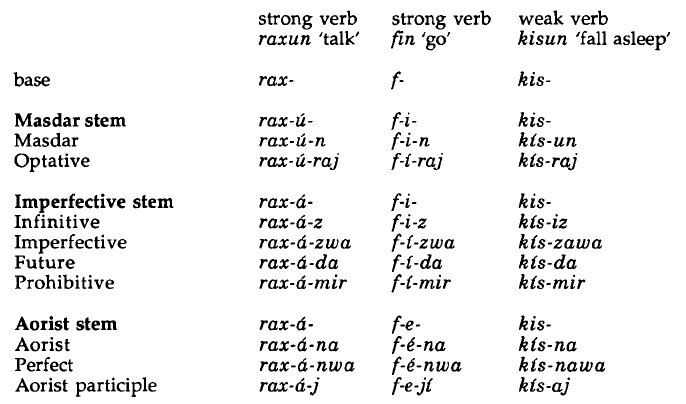
\includegraphics{Lezgian/src/verb.png}
\end{center}
\subsection{강동사의 세 어간}
강동사 어간은 보통 동사 어기에 모음을 접미시켜 만드나, 일부는 보충법으로 형성된다. 어간말 모음은 어간 모음과의 모음조화 및 순장애음-모음 조화를 통해 결정되므로 고저만이 변별적이다. 마스다르 어간은 항상 고모음(U)이나, 미완료와 부정과거 어간은 저모음(A)일 수 있으며, 가능한 조합이 모두 나타난다. 추가로 \textit{u-i-a} 패턴이 있으며, 일부 동사는 어간 모음까지 교체되기도 한다. 
\subsection{동사 굴절 범주}
비정형에는 분사, 부동사, 부정사, 마스다르, 그리고 우언법 형태가 속하며, 나머지는 정형이고 그 중에서 권고법, 기원법, 조건법, 금지법이 비-직설법이다. 다음의 목록을 참조.
\begin{center}
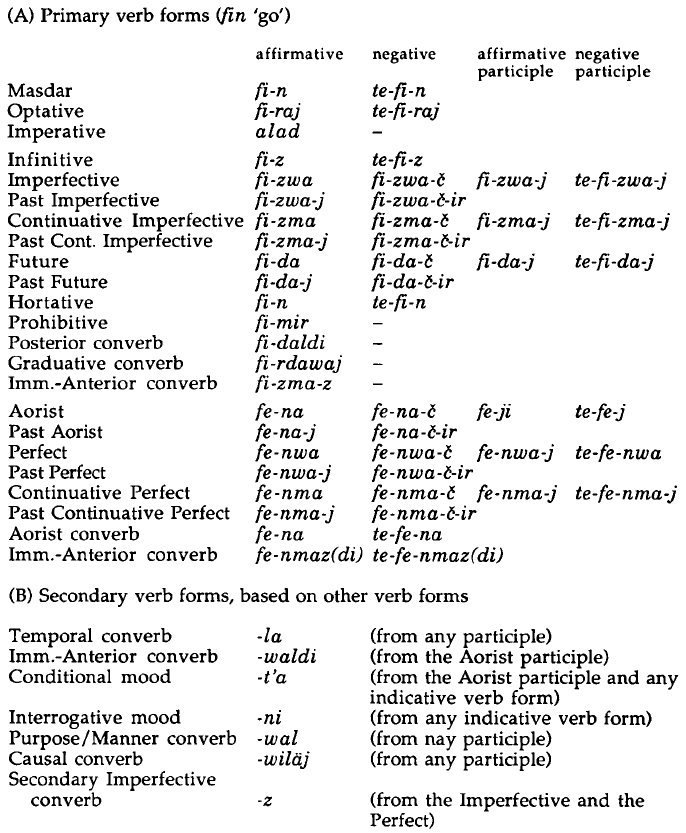
\includegraphics{Lezgian/src/veri.png}
\end{center}
공통적으로 비과거 직설법 형태의 과거형은 긍정에서 \textit{-j}(부정과거를 제외한 분사도 동일하게 형성), 부정에서 (상 접미사 뒤에 붙는 부정 접미사 \textit{-č} 뒤에) \textit{-ir}를 접미시켜 만든다. 비정형, 권고법, 기원법의 부정형은 접두사 \textit{tV-}나 우언법으로 만든다.
\subsubsection{마스다르 어간에서 파생된 형태}
\begin{enumerate}
	\item \textbf{마스다르(동명사)}는 강동사에 \textit{-n}, 약동사에 \textit{-un}을 붙여 만들며, 격과 수에 따라 굴절한다(사격 어간 \textit{-i}, 복수형 \textit{-ar}). 어기에 자음이 하나뿐인 몇몇 동사는 C-V-n-V-C 형식의 2차적 마스다르 형태가 있다. 예컨대 \textit{fi-n-if} '감'.
	\item \textbf{기원법} 접미사는 \textit{-raj}이며, 드물게 \textit{-j/-uj}가 쓰인다.
	\item \textbf{명령법}을 만드는 방식에는 여러 가지가 있는데,
	\begin{itemize}
		\item 대부분의 강동사는 어간의 마지막 자음을 반복한다. 그 자음이 \textit{r}이면 첫 자음을 대신 반복한다.
		\item 접미사 \textit{-r}로 만드는 동사가 네 개, 마스다르 어간 그대로인 동사가 세 개 있으며 보충법(예컨대 \textit{fi-n} $\rightarrow$ \textit{alad} '가라')이나 다른 불규칙형으로 나타나는 동사들도 존재한다.
		\item 대부분의 약동사는 어기를 그대로 명령형으로 쓰든지, 특히 \textit{-r}로 끝나거나 \textit{awun} 합성어이거나 대응하는 역사동형이 있는 경우에 필수적인 \textit{-a} 접미사를 붙여 사용한다.
	\end{itemize}
\end{enumerate}
\subsubsection{미완료 어간에서 파생된 형태}
\begin{enumerate}
	\item \textbf{부정사(미완료 부동사)} 접미사는 \textit{-z/-iz}이며, 부동사는 간혹 중첩된다는 것 외에 두 기능의 형태적 차이는 없다. 마스다르와 달리 명사 곡용을 하지 않는다.
	\item \textbf{미완료} 접미사는 \textit{-zwa/-zawa}이며, 미완료 부동사 + 장소계사 \textit{awa}로 비교적 최근에 형성된 형태이다.
	\item \textbf{계속적 미완료} 접미사는 \textit{-zma/-zama}이며, 미완료 부동사 + 계속상 계사 \textit{ama}의 조합이다.
	\item \textbf{미래} 접미사는 \textit{-da}로, 습관상의 기능도 갖는다. 이는 미완료 형태가 생겨나 진행상과 일반적 현재의 의미를 빼앗자, 기존의 비과거에서 미래와 습관상의 의미만 남은 결과로 보인다. 이는 일부 상태동사가 현재형으로 \textit{-da}를 쓰는 것에서도 나타난다.
	\item \textbf{권고법} 접미사는 \textit{-n/-in}이다.
	\item \textbf{금지법} 접미사는 \textit{-mir}이며, 이것은 \textit{awun} '하다'의 옛 금지형 \textit{m-iji-r} '하지 마라'에서 문법화된 것으로 보인다.
	\item \textbf{후행적 부동사} 접미사는 \textit{-daldi}이고, 미래 시제에서 파생되었다고 추측되며, 종종 '-까지'의 뜻으로 쓰이는 상분리격 \textit{-ldi}와 관련있다.
	\item \textbf{점진적 부동사} 접미사는 \textit{-rdawaj/-irdawaj}이다.
	\item \textbf{직전-선행적 부동사} 접미사는 \textit{-zmaz/-zamaz}이다.
\end{enumerate}
\subsubsection{부정과거 어간에서 파생된 형태}
\begin{enumerate}
	\item \textbf{부정과거} 접미사는 \textit{-na}이며, 긍정형은 상응하는 부동사와 동음이의이다.
	\item \textbf{부정과거 분사} 접미사는 약동사에서 \textit{-aj}(드문 고어형으로 \textit{-ur}), 강동사에서 \textit{-r/-j/-ji}이며, 후자는 각각 어간말 고모음, 다음절 어간말 저모음, 단음절 어간말 저모음 뒤에서 쓰인다.
	\item \textbf{완료와 계속적 완료} 접미사는 각각 \textit{-nwa/-nawa}와 \textit{-nma/-nama}이다. 기원에 관해서는 미완료와 계속적 미완료를 참조. 계속적 완료는 문법화 정도가 덜해 어중 모음 탈락이 일어나지 않은 형태도 관찰된다.
	\item \textbf{부정과거 부동사} 접미사는 \textit{-na}이다.
	\item \textbf{직전-선행적 부동사} 접미사는 \textit{-nmaz(di)/-namaz(di)}이다.
\end{enumerate}
\subsubsection{2차적 동사 범주}
\begin{enumerate}
	\item \textbf{시간적 부동사} 접미사는 \textit{-la}이며 모든 분사에서 파생 가능하다.
	\item \textbf{직전-선행적 부동사} 접미사는 \textit{-waldi}이며 부정과거 분사에서 파생된다.
	\item \textbf{조건법} 접미사는 \textit{-t'a}이며 모든 직설법 동사와 부정과거 분사에 붙을 수 있다(부정과거 분사에 붙는 것이 일반적이다). 다른 비정형 동사 형태들과 마찬가지로 초점 표지 \textit{-ni} '-도'가 붙을 수 있으며 양보적 관계를 표현한다.
	\item \textbf{의문법} 접미사는 \textit{-ni}이며, 모든 직설법 동사에 붙을 수 있다.
	\item \textbf{2차적 미완료 부동사} 접미사는 \textit{-z}이며, 완료나 계속적 완료 혹은 미완료 동사형 뒤에 올 수 있다.
	\item \textbf{의도/방식 부동사} 접미사는 추상명사 접미사와 동음이의인 \textit{-wal}이며, 모든 분사형에 붙을 수 있다.
	\item \textbf{인과적 부동사} 접미사는 기원적으로 추상명사 접미사의 내분리격 형태인 \textit{-wiläj}이며, 모든 분사형에 붙을 수 있다.
\end{enumerate}
\subsubsection{접두적 부정negation 및 우언법periphrasis 형태}
비정형 및 비-직설법 동사는 접두적으로 부정된다. 대부분의 경우에 이는 부정 조동사 \textit{t-awun} '하지 않다'를 아용한 우언적 부정이지만, 한정된 수의 동사들은 직접 \textit{t(A)-}를 받는다. 해당하는 동사는 다음과 같다.
\begin{center}
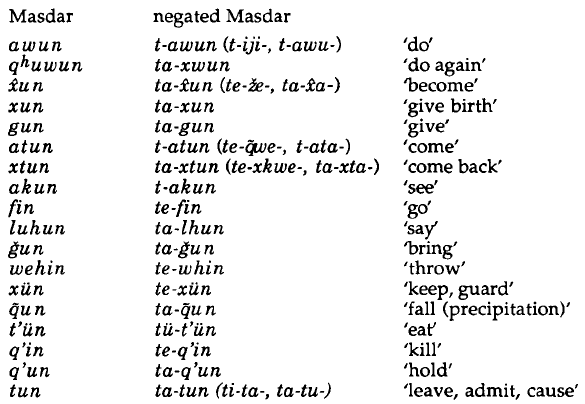
\includegraphics{Lezgian/src/prne.png}
\end{center}
모두 강동사이며 대부분 단음절이다. 이에 해당하는 동사들은 시간이 지날수록 줄어들고 있다.
\begin{itemize}
	\item 우언법 형태는 약동사는 동사 어기와 같고 강동사는 대부분 마스다르 형태와 같다.
	\item 미완료 어간 동사형과 결합한 강동사의 우언법 형태는 수의적으로 권고법 형태와 같을 수 있다. 이러한 분포는 우언적 반복형, 또는 동사 어기가 초점 표지 \textit{-ni} '-도'로 표시되는 경우에도 나타나는 것이다.
\end{itemize}
\begin{center}
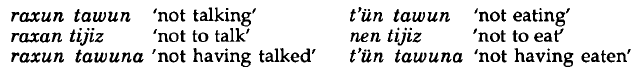
\includegraphics{Lezgian/src/peri.png}
\end{center}
\subsection{부분적인 패러다임 예시}
\omission
\subsection{불규칙 동사}
\subsubsection{계사}
\begin{itemize}
	\item 기본 계사 \textit{ja} '-이다'와 다섯 가지 장소 계사 \textit{awa} '안에 있다', \textit{gwa} '옆에 있다', \textit{gala} '뒤에 있다', \textit{kwa} '아래에 있다', \textit{ala} '위에 있다'(및 각각의 계속상 변이형 \textit{ama, guma, galama, kuma, alama})는 불완전 활용을 한다.
	\item 현재 시제, \textit{-j}로 만드는 과거 시제와 분사, 접미적 부정형 \textit{-č}, 부동사형 \textit{-z}이 존재하며, 미완료, 미래, 부정과거 어간 기반의 모든 형태, 마스다르 형태가 없다.
	\item 계사는 또한 부동사와 그 분사에서도 \textit{-ir}로 만드는 접미적 부정형을 갖는다.
	\item 기본 계사는 보충형도 갖는다.
\end{itemize}
\begin{center}
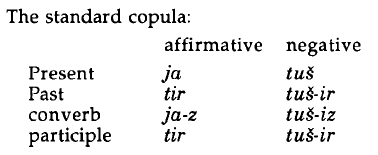
\includegraphics{Lezgian/src/stco.png}
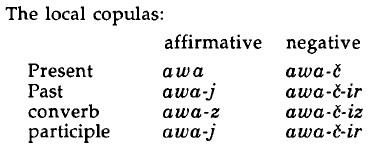
\includegraphics{Lezgian/src/loco.png}
\end{center}
\subsubsection{마스다르 및 부정과거 어간이 없는 동사}
다음의 동사들은 마스다르 및 부정과거 어간이 없으며, 미래형 \textit{-da}가 비-미래, 비-습관상, 현재 상태 의미를 갖는다는 점에서 공통적이다. 이 동사들의 나머지 활용형은 \textit{x̂un} '되다'를 빌어 나타낸다.
\begin{enumerate}
	\item \textbf{\textit{k'an} '사랑하다, 필요하다, 원하다'}는 형용사 \textit{k'an} '사랑하는'에서 나왔으며, 미완료 \textit{k'anzawa}, 미래 \textit{k'anda}, 부동사 \textit{k'anz} 형태가 있고 추가로 어간 + 계사 형식이 쓰인다. 관형형 \textit{k'ani}(부정형 \textit{tek'ani})도 있다.
	\item \textbf{\textit{kič'e} '두려워하다'} 역시 기원적으로 형용사이다. 관형적으로도 쓰이나 접두적 부정형은 없다.
	\item \textbf{\textit{či-} '알다'}는 관형형이 없는 대신 우언법 형태 \textit{čin}이 있다.
	\item \textbf{\textit{t'a-} '아프다'}
\end{enumerate}
\subsubsection{\textit{-ä(ǧ)-}로 끝나는 어간의 동사}
\begin{center}
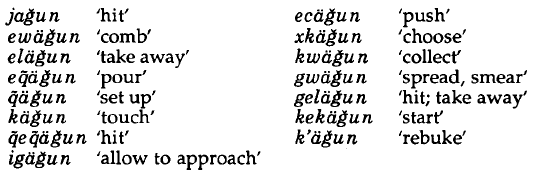
\includegraphics{Lezgian/src/agve.png}
\end{center}
이 동사들은 ǧ가 음절말, 즉 어말이나 자음으로 시작하는 접미사 앞에 오게 되면 탈락한다.  
\subsection{기본적인 시제-시상 범주의 기능}
기본 네 개의 시상 범주(미완료, 미래, 부정과거, 완료)에 더해 계속상(미완료나 완료와 결합해서만 나타남)과 과거(나머지 시제-시상 범주와 결합해서 나타남) 총 여섯 가지가 있다.
\subsubsection{미완료}
보통 해당 시점에 진행 중인 상황을 나타내나, 해당 시점에 존재하는 상태를 나타내기도 한다는 점에서 통상적인 진행상과 다르다. 습관적 상황도 나타내는데, 구어에서는 미래보다 선호된다.
\subsubsection{미래}
미래의 상황을 나타내거나 습관적 상황을 나타내는 두 가지 다른 용법이 있으며, 구어에서는 전자가 지배적이고, 후자는 형식적인 문체나 속담에서 사용된다. 습관상 의미에만 과거가 호환되지만, '과거 미래'는 가정적 용법도 갖고 있다. 일부 불규칙 동사에서는 현재의 상태를 나타내며, 극의 지문에도 쓰인다.
\subsubsection{부정과거aorist}
과거의 완료적 사건을 나타내는 데에는 보통 부정과거가 쓰인다. 또한 서사에서 쓰이는 범주이기도 하다. '과거 부정과거'는 먼 과거의 상황이나, 주 줄거리 전에 일어난 상황, 더 이상 존재하지 않는 상황, 영향력이 사라진 상황 등을 나타낸다.
\subsubsection{완료}
'새로운 소식'과 같이 현재와 관련이 있는 과거의 사건에 대해 쓰인다. 많은 동사에서 완료는 귀결적인 의미, 즉 과거 사건의 결과로서의 상태를 나타내는데, 자세 동사가 대표적이다. 과거 완료는 다른 과거 상황에 대해 시간적 선행성을 표현한다.
\subsubsection{계속적 미완료 및 완료}
계속상은 미완료나 완료와 결합해 '여전히'(부정은 '더 이상 -- 아니다')의 의미를 더하며, 때로 부사 \textit{hele} '여전히'가 잉여적으로 쓰인다. 계속상이 완료와 결합하면 완료는 귀결적 의미만 가질 수 있다.
\subsubsection{과거past}
과거는 다른 시제-시상 범주와 결합해서만 나타난다.
\subsection{우언적 시제-시상 범주}
\subsubsection{우언적 습관}
우언적 습관은 조동사 \textit{x̂un} + 부정사로 만들며, 이때 조동사는 원래 습관상의 의미를 갖는 미래일 필요는 없다. 예컨대 \textit{qaču-z x̂un} '가져가곤 하다'.
\subsubsection{우언적 미래}
우언적 미래는 계사 + 미래 분사에서 파생된 의도/방식 부동사로 만들며, 종종 (종합적 미래보다 더) 직후의 미래를 표현한다. 예컨대 \textit{qaču-da-j-wal ja} '가져가겠다'. \textit{tir}나 \textit{x̂ana} 등 계사의 과거 시제와 결합하면, 과거 시점에서의 직후 미래를 표현하며, '과거 미래'와 같이 가정적 의미도 가질 수 있다.
\subsubsection{전언 증거}
전언 증거는 (비-부정 비-과거) 정형 직설법 동사형에 접미사 \textit{-lda}를 붙여 만든다. 이는 \textit{luhuda} '(누가) 말한다'의 축약과 접미로 최근에 문법화된 것이다.
\subsection{비-직설법 정형 동사 형태의 기능}
\subsubsection{명령법}
명령, 요청, 훈계 등의 의미를 가지며, 부정형 대신 금지법을 사용한다. 때로는 (청자의 수를 명확히 하고 싶은 경우 등) 2인칭 주어가 생략되지 않는 경우도 있다.
\subsubsection{금지법}
금지법은 부정 명령법과 같다.
\subsubsection{권고법}
권고법은 1인칭 단/복수 청자에게 권고하는 의미로, 종종 문두 소사 \textit{ša} '와라'가 함께 쓰인다. 권고법은 또한 의도 질문(화자가 자기 자신이 할 행동에 대해 묻는 것)에도 쓰인다. 종종 \textit{belki} '아마'와 함께 불확실한 진술이나 질문에도 쓰이며, 이 경우 주어가 2/3인칭 명사구일 수 있다. 
\subsubsection{기원법}
기원법은 운명이나 신이 결정할 수 있는 것에 대한 기원을 나타낸다. 또한 3인칭 행동주에 대한 권고에도 쓰인다. 두 기능 모두에 대해 문두 소사 \textit{quj}가 종종 함께 나온다. 서약이나 권고법과 같이 의도 질문에도 사용된다.
\subsubsection{조건법}
조건법은 조건절, 양보절, 간접 의문문, 상관적 관계절에 쓰인다. 해당 장들을 참조.
\subsubsection{의문법}
의문법은 선택 의문문과 직접 판정 의문문에 쓰인다.
\subsection{비정형 동사 형태의 기능}
\subsubsection{마스다르(동명사)}
마스다르는 관례적으로 동사의 표제형이며, 행동의 명사화이다. 예컨대 \textit{aqwaz-un} '멈춤'. 형태와 분포는 명사적이지만, 수식이나 논항 결합 등의 면에서는 동사이다. 사실보다는 상황을 나타내는 경우가 더 흔하다. 명사적 마스다르도 존재하는데, 이 경우에는 복수형 등 모든 면에서 명사적이며 보통 결과물의 의미를 갖는다.
\subsubsection{분사}
분사는 관계절을 만들며, 형용사처럼 실질화되어 핵어 없는 관계절을 만들 수도 있다. 분사의 시제-시상 범주는 해당하는 정형동사의 그것과 보통 일치한다. 부정과거 분사의 경우 조건 표지 \textit{-t'a}가 붙을 수 있다.
\subsubsection{부정사infinitive}
부정사는 보문절과 의도절, 또는 의미적으로 불특정한 부사절에 쓰일 수 있다(미완료 부동사). 후자는 보통 동시적 부대상황을 표현한다.
\subsubsection{부정과거 부동사}
부정과거 부동사 역시 불특정한 부사적 종속절로 쓰이나, 주절의 사건보다 앞선 사건을 나타낸다.
\subsubsection{특수 부동사}
후행적, 점진적, 시간적, 인과적, 의도/방식, 직전-선행적 부동사 등의 용법은 21장을 참조.
\subsection{고어 형태}
Uslar (1896)에 기술된 시제-시상 범주 중 세 가지 및 미완료 분사형 하나는 현대 표준어에 나타나지 않는다.
\subsubsection{고어형 과거preterit}
부정과거 어간에 접미사 \textit{-ra}나 \textit{-ja/-aja}를 붙여 만든다. 부정과거 분사에 접미사 \textit{-a}를 붙여 파생시킨 것으로 보인다. 부정형은 \textit{-nč}로 끝난다. Uslar에 따르면 고어형 과거는 놀란 뉘앙스를 준다는 점에서 부정과거와 약간 다르다.
\subsubsection{고어형 미래}
미완료 어간에 접미사 \textit{-di}(부정형 \textit{-(i)č})를 붙여 만든다. Uslar에 따르면 미래 사건에 대해 덜 단언적이며 주로 조건문의 귀결절에 나타난다. 고어형 과거처럼 완전히 사라지지는 않았으며, 부정형으로나 동사 \textit{x̂un}과 함께 나타난다. 
\subsubsection{고어형 과거 미래}
미완료 어간에 접미사 \textit{-dir}(부정형 \textit{-čir})를 붙여 만든다. 가정적 조건문의 귀결절에 나타난다고 한다.
\subsubsection{고어형 미완료 분사}
오늘날에는 미완료 분사가 정령 미완료형에서 파생되나, 이전 시기에는 미완료형 어간에 바로 접미사 \textit{-r/-ri}를 붙여 만드는 규칙적 미완료 분사가 있었을 것이다. 발견한 예시는 모두 강동사이다.
\begin{center}
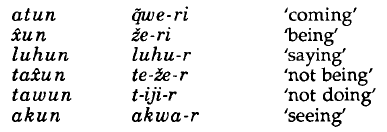
\includegraphics{Lezgian/src/impa.png}
\end{center}
다음과 같이 두 개의 고어형 미완료 분사를 이어붙여 만드는 구문이 존재한다.
\begin{center}
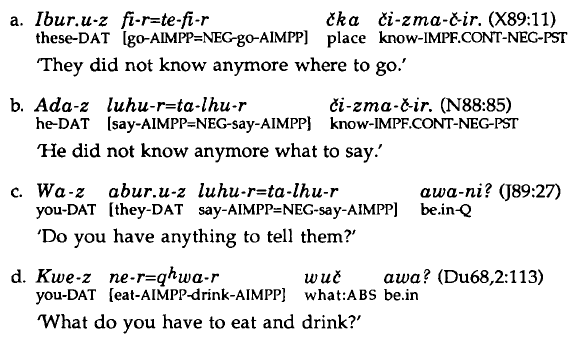
\includegraphics{Lezgian/src/papa.png}
\end{center}














